\bigskip

\item Which of these functions has an inverse?

% \bigskip
% 
% (a)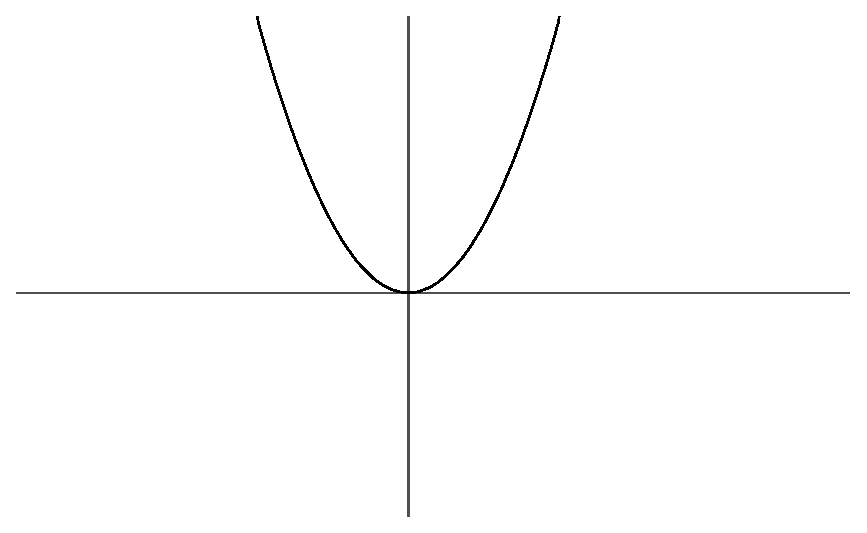
\includegraphics[height=90pt]{SVC.01.03.051a.eps}(b)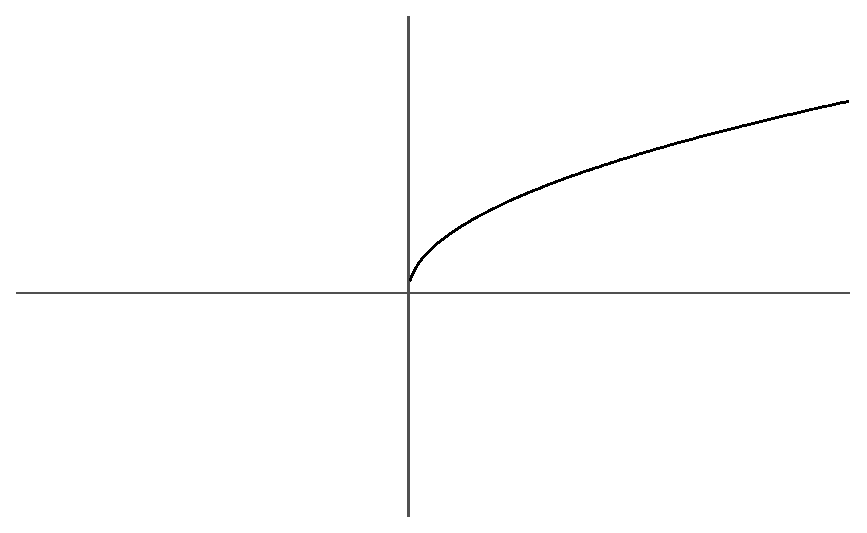
\includegraphics[height=90pt]{SVC.01.03.051b.eps}\\
% (c)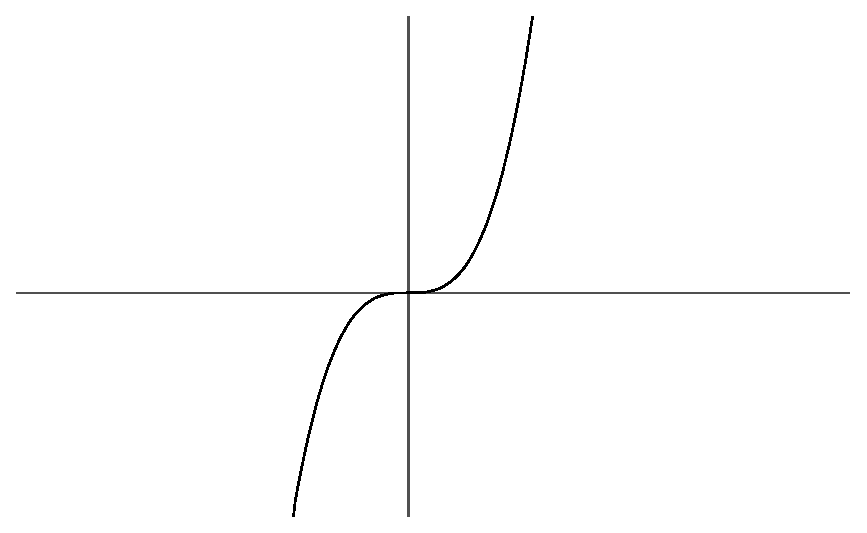
\includegraphics[height=90pt]{SVC.01.03.051c.eps}(d)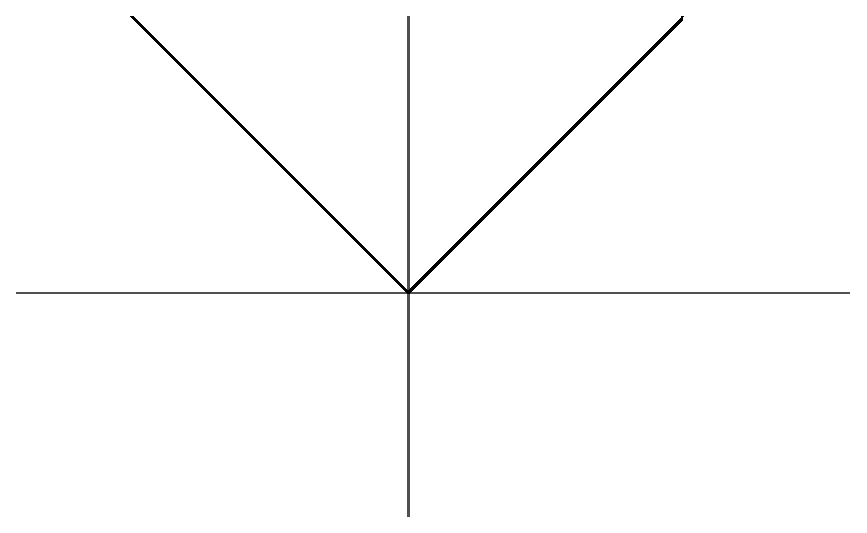
\includegraphics[height=90pt]{SVC.01.03.051d.eps}
    \begin{tikzpicture}
        \begin{axis}[axis lines=center, xlabel={$x$}, ylabel={$y$}, xmin=-3, xmax=3,
                ymin=-3, ymax=3, xtick=\empty, ytick=\empty, yticklabels={},
            xticklabels={}, title={Plot (a)}]
                \addplot[color=blue, very thick] {(1/3)*x^2};
            \end{axis}
        \end{tikzpicture}
    \begin{tikzpicture}
        \begin{axis}[axis lines=center, xlabel={$x$}, ylabel={$y$}, xmin=-3, xmax=3,
                ymin=-3, ymax=3, xtick=\empty, ytick=\empty, yticklabels={},
            xticklabels={}, title={Plot (b)}]
                \addplot[color=blue, very thick,domain=0:3,samples=100] {sqrt(x)};
            \end{axis}
        \end{tikzpicture}\\
    \begin{tikzpicture}
        \begin{axis}[axis lines=center, xlabel={$x$}, ylabel={$y$}, xmin=-3, xmax=3,
                ymin=-3, ymax=3, xtick=\empty, ytick=\empty, yticklabels={},
            xticklabels={}, title={Plot (c)}]
                \addplot[color=blue, very thick,domain=-3:3] {(1/9)*x^3};
            \end{axis}
        \end{tikzpicture}
    \begin{tikzpicture}
        \begin{axis}[axis lines=center, xlabel={$x$}, ylabel={$y$}, xmin=-3, xmax=3,
                ymin=-3, ymax=3, xtick=\empty, ytick=\empty, yticklabels={},
            xticklabels={}, title={Plot (d)}]
                \addplot[color=blue, very thick,domain=-3:3] {abs(x)};
            \end{axis}
        \end{tikzpicture}

\begin{enumerate}
\item (a) only
\item (b) only
\item (c) only
\item (d) only
\item (a) and (b)
\item (b) and (c)
\end{enumerate}
%by Project MathVote
